% ============================================================
%  CHAPITRE 2 — Section : Analyse de robustesse face aux défaillances
% ============================================================

\subsection{Robustesse face aux défaillances}
\label{sec:robustesse}

Le plan de Pareto de la sous-section précédente a caractérisé le comportement nominal des stratégies, lorsque tous les composants sont opérationnels. Il ne dit rien de leur comportement lorsqu'un composant tombe en panne, situation pourtant inévitable sur la durée de vie d'un système isolé et dépourvu de tout secours extérieur. Cette sous-section éprouve la troisième dimension de performance, la robustesse, c'est-à-dire la capacité d'une EMS à maintenir le service en présence d'une défaillance temporaire d'un organe de stockage. L'indicateur de robustesse (équation~\eqref{eq:indic_robustesse}), les scénarios de défaillance et le protocole d'évaluation par Monte-Carlo ayant été définis à la section~\ref{subsec:indic_robustesse}, cette sous-section en présente et en analyse les résultats.

% ------------------------------------------------------------
\subsubsection{Résultats}
\label{subsec:rob_resultats}
% ------------------------------------------------------------

La Figure~\ref{fig:rob_boxplots} présente la distribution de la LPSP sous défaillance pour chaque stratégie et chaque scénario, le repère rouge indiquant la LPSP moyenne en marche normale (l'écart au losange noir matérialisant le surcoût lié à la défaillance). La Figure~\ref{fig:rob_heatmap} en synthétise la LPSP moyenne, et la Figure~\ref{fig:rob_heatmap_delta} le surcoût de robustesse moyen, c'est-à-dire l'effet propre de la panne, débarrassé de la variabilité du profil de charge.

\begin{figure}[h!]
    \centering
    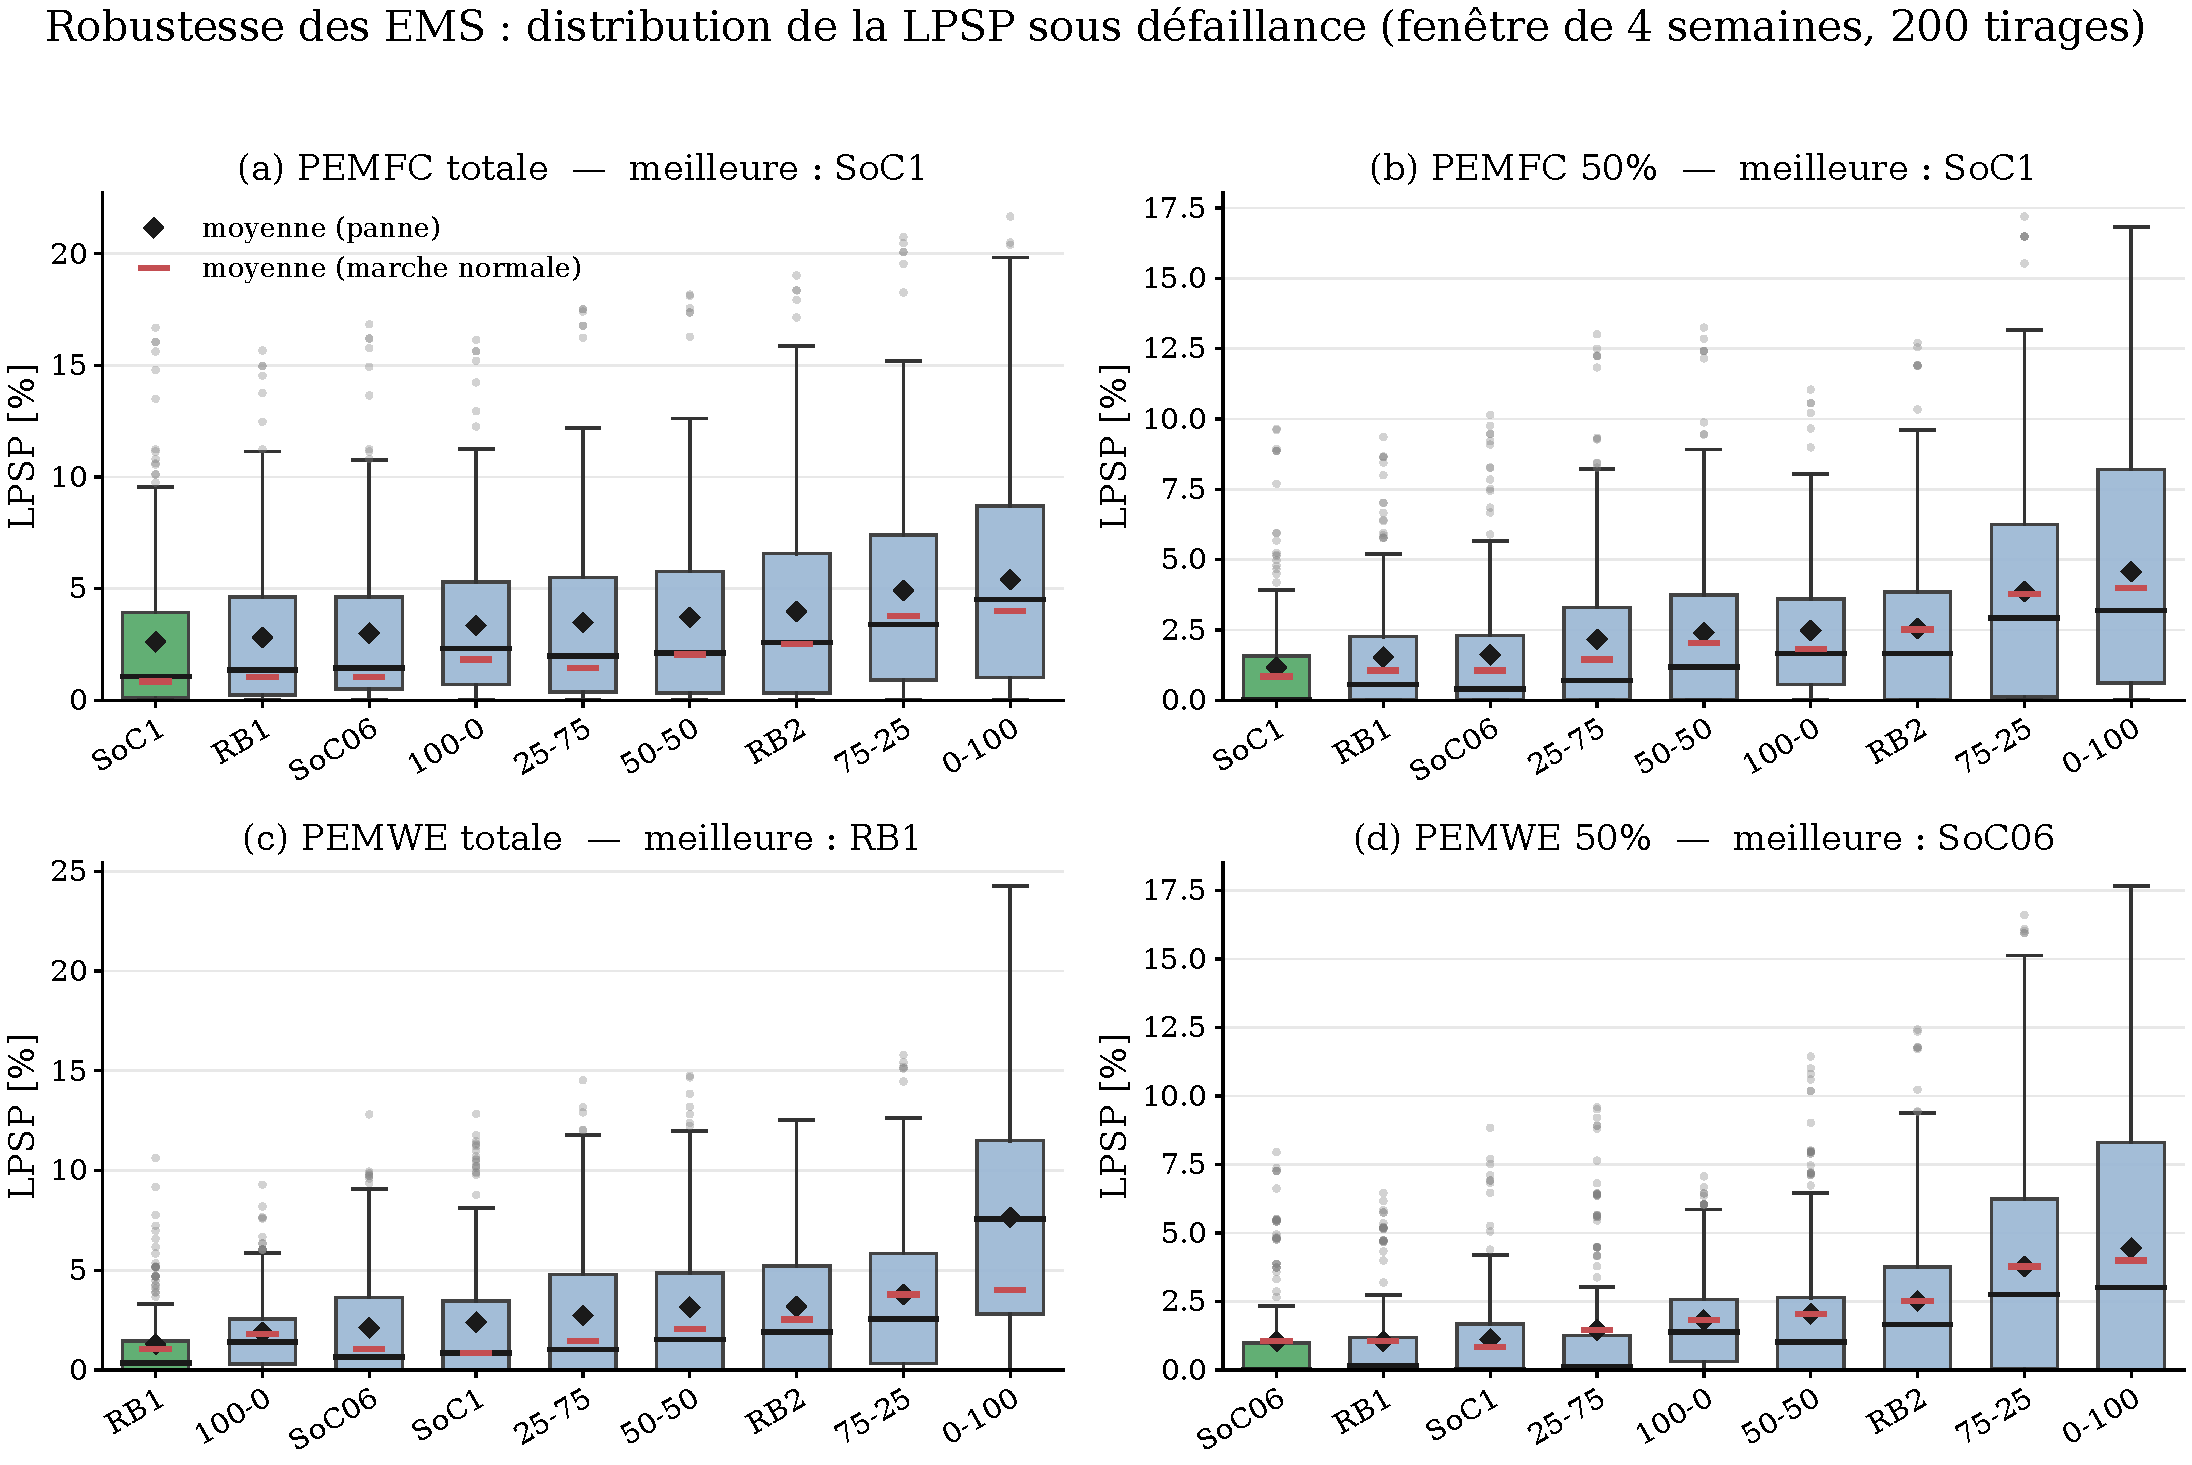
\includegraphics[width=\linewidth]{Chapitre 2/Robustesse/Figures/robustesse_boxplots.pdf}
    \caption{Distribution de la LPSP sous défaillance, par stratégie et par scénario (fenêtre de 4~semaines, 200~tirages).}
    \label{fig:rob_boxplots}
\end{figure}
\FloatBarrier

\begin{figure}[h!]
    \centering
    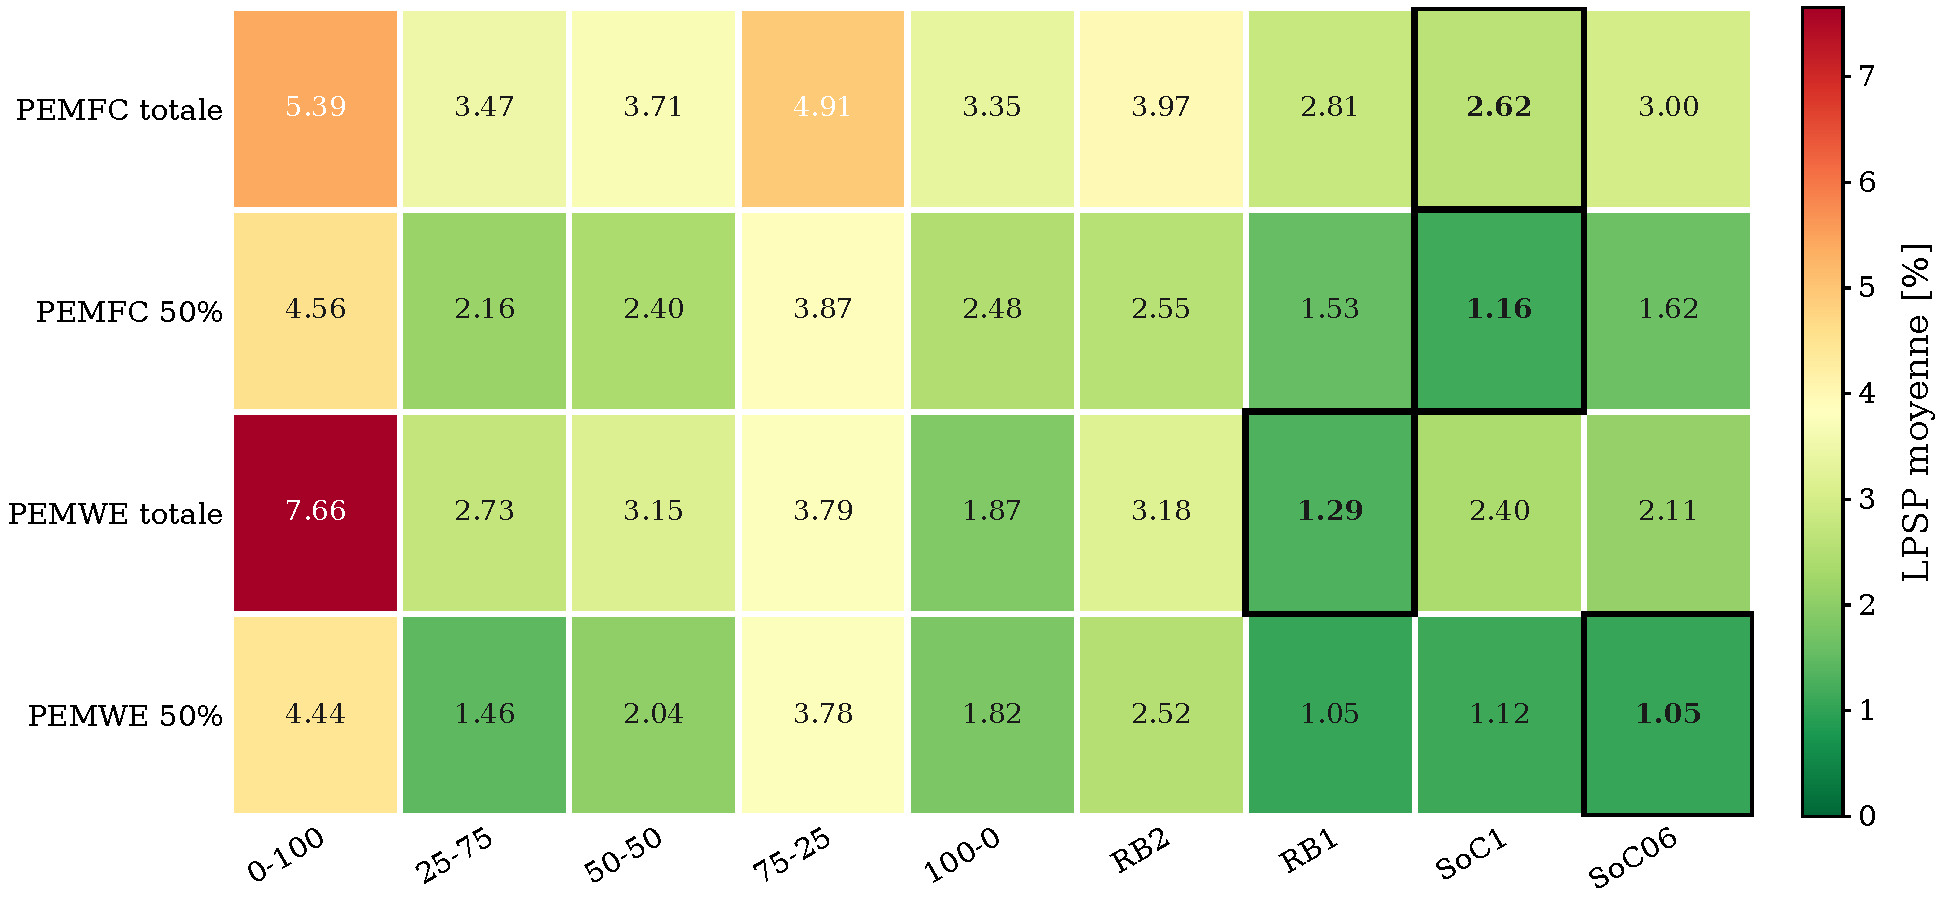
\includegraphics[width=\linewidth]{Chapitre 2/Robustesse/Figures/robustesse_heatmap.pdf}
    \caption{LPSP moyenne sous défaillance (scénario $\times$ stratégie). La cellule la plus favorable de chaque ligne est encadrée.}
    \label{fig:rob_heatmap}
\end{figure}
\FloatBarrier

\begin{figure}[h!]
    \centering
    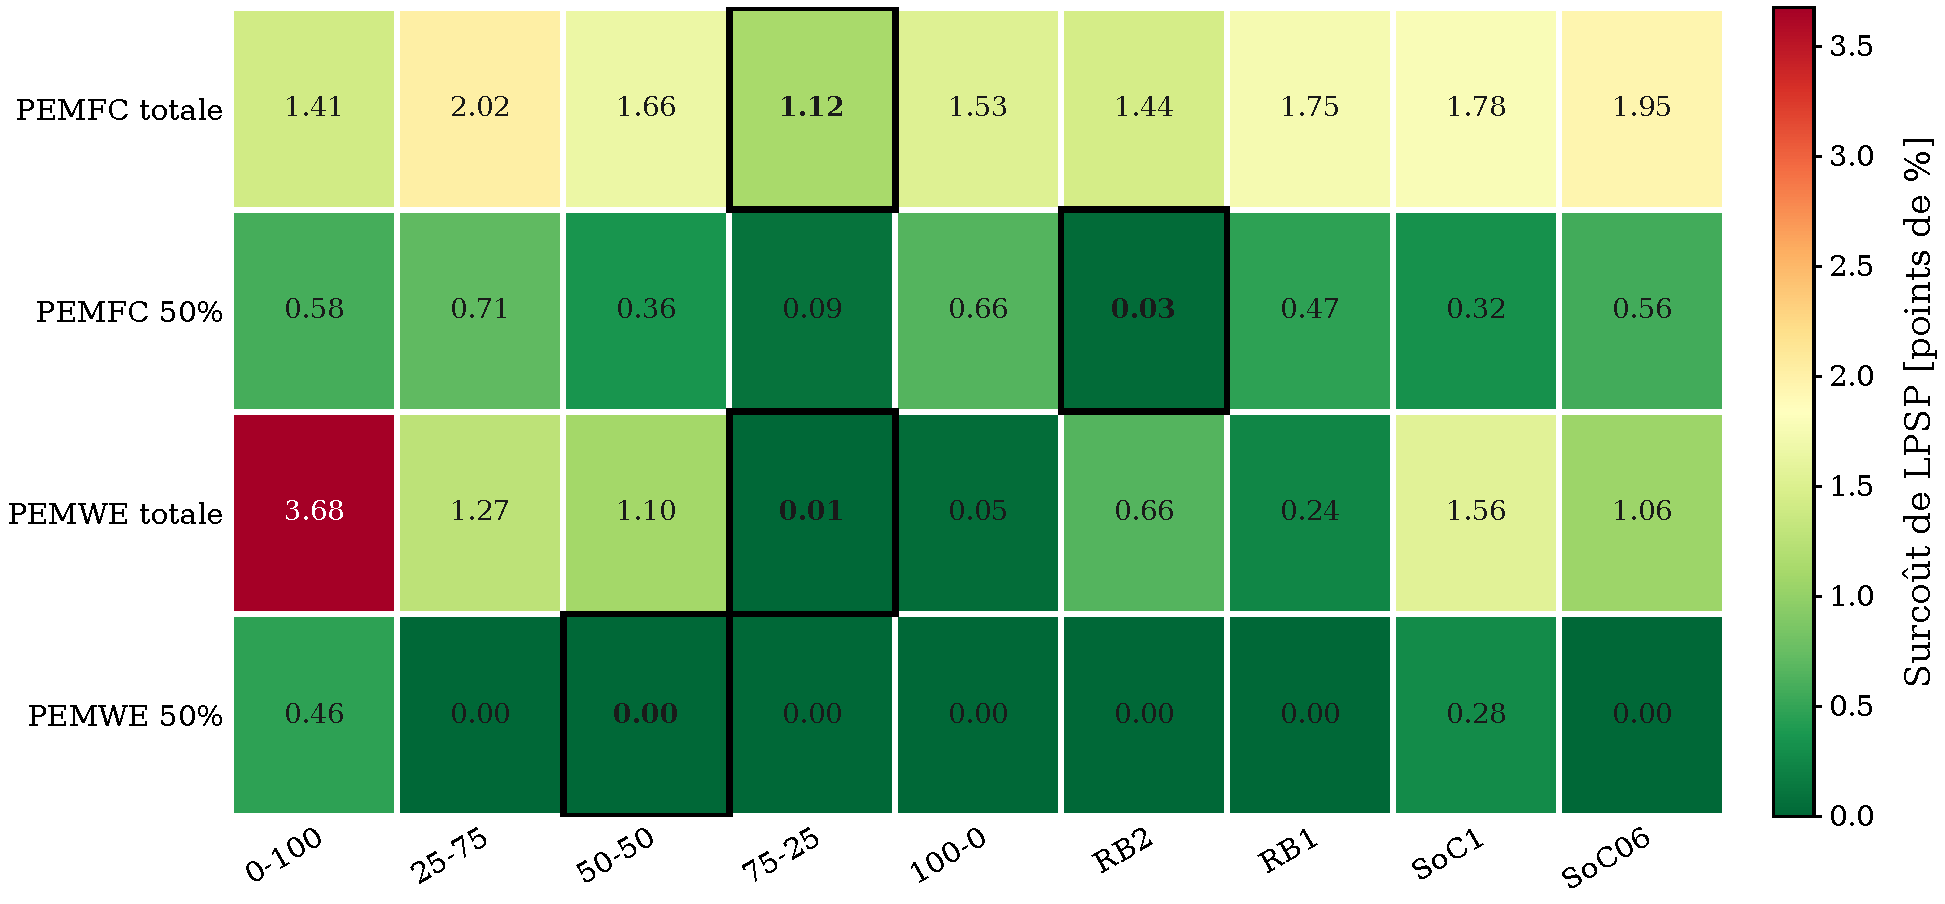
\includegraphics[width=\linewidth]{Chapitre 2/Robustesse/Figures/robustesse_heatmap_delta.pdf}
    \caption{Surcoût de défaillance $\Delta\mathrm{LPSP}_{\text{rob}} = \mathrm{LPSP}(\text{panne}) - \mathrm{LPSP}(\text{marche normale})$, en points de pourcentage.}
    \label{fig:rob_heatmap_delta}
\end{figure}
\FloatBarrier

En LPSP absolue (Figure~\ref{fig:rob_heatmap}), les stratégies maintenant une forte réserve de batterie s'en sortent le mieux. SoC1 minimise la LPSP en cas de défaillance de la pile à combustible (\SI{2{,}62}{\percent} en panne totale, \SI{1{,}16}{\percent} en panne partielle), tandis que RB1 et SoC06 dominent en cas de défaillance de l'électrolyseur (respectivement \SI{1{,}29}{\percent} pour la PEMWE totale et \SI{1{,}05}{\percent} pour la PEMWE \SI{50}{\percent}). Ce résultat est en partie trompeur, car ces stratégies présentent déjà une faible LPSP nominale (forte réserve d'énergie disponible)~: leur bonne tenue en panne reflète davantage leur fonctionnement de base que leur réaction propre à la défaillance.

Une fois isolé l'effet propre de la panne (Figure~\ref{fig:rob_heatmap_delta}), le classement change. Les stratégies à dominante batterie (75-25, 100-0, RB2) affichent les surcoûts les plus faibles, inférieurs à un dixième de point pour la défaillance partielle de la pile à combustible. À l'inverse, la stratégie « tout-hydrogène » 0-100 se dégrade fortement dès qu'un composant hydrogène défaille~: son surcoût atteint \SI{3{,}66}{} points en cas de panne totale de l'électrolyseur (LPSP moyenne de \SI{7{,}65}{\percent}, soit le pire cas observé), ce qui traduit une dépendance excessive au sous-système hydrogène et une absence de marge de repli. La défaillance partielle de l'électrolyseur (PEMWE \SI{50}{\percent}) engendre quant à elle des surcoûts quasi nuls pour la plupart des stratégies, le surplus PV non absorbé étant simplement réorienté vers la batterie, sans perte de service immédiate.

Le meilleur choix dépend donc du scénario considéré~: une défaillance de la pile à combustible est le mieux encaissée par les stratégies maintenant une forte réserve de batterie (SoC1), tandis qu'une défaillance de l'électrolyseur l'est par celles qui préservent une marge de charge (RB1, SoC06). Aucune stratégie ne minimise la LPSP dans tous les scénarios à la fois~: ce qui distingue les stratégies, c'est le composant dont elles dépendent et la marge de repli qu'elles conservent.

La LPSP moyenne ne dit rien de la dispersion des situations selon l'instant de la panne. Or, pour un système isolé, ce sont souvent les pires cas qui dimensionnent l'acceptabilité du service. La Figure~\ref{fig:rob_cdf} présente, pour chaque scénario, les fonctions de répartition de la LPSP sous défaillance. Leur lecture confirme et précise les conclusions précédentes~: les stratégies préservant une réserve de batterie présentent non seulement une LPSP moyenne plus faible, mais aussi des queues de distribution nettement plus courtes, c'est-à-dire des coupures maximales bien moindres lorsque la panne tombe au plus mauvais moment. À l'inverse, la courbe de l'EMS 0-100 s'étire loin vers la droite, traduisant des épisodes de coupure sévères (jusqu'à plus de \SI{24}{\percent} de LPSP sur la fenêtre en cas de panne totale de l'électrolyseur).

\begin{figure}[h!]
    \centering
    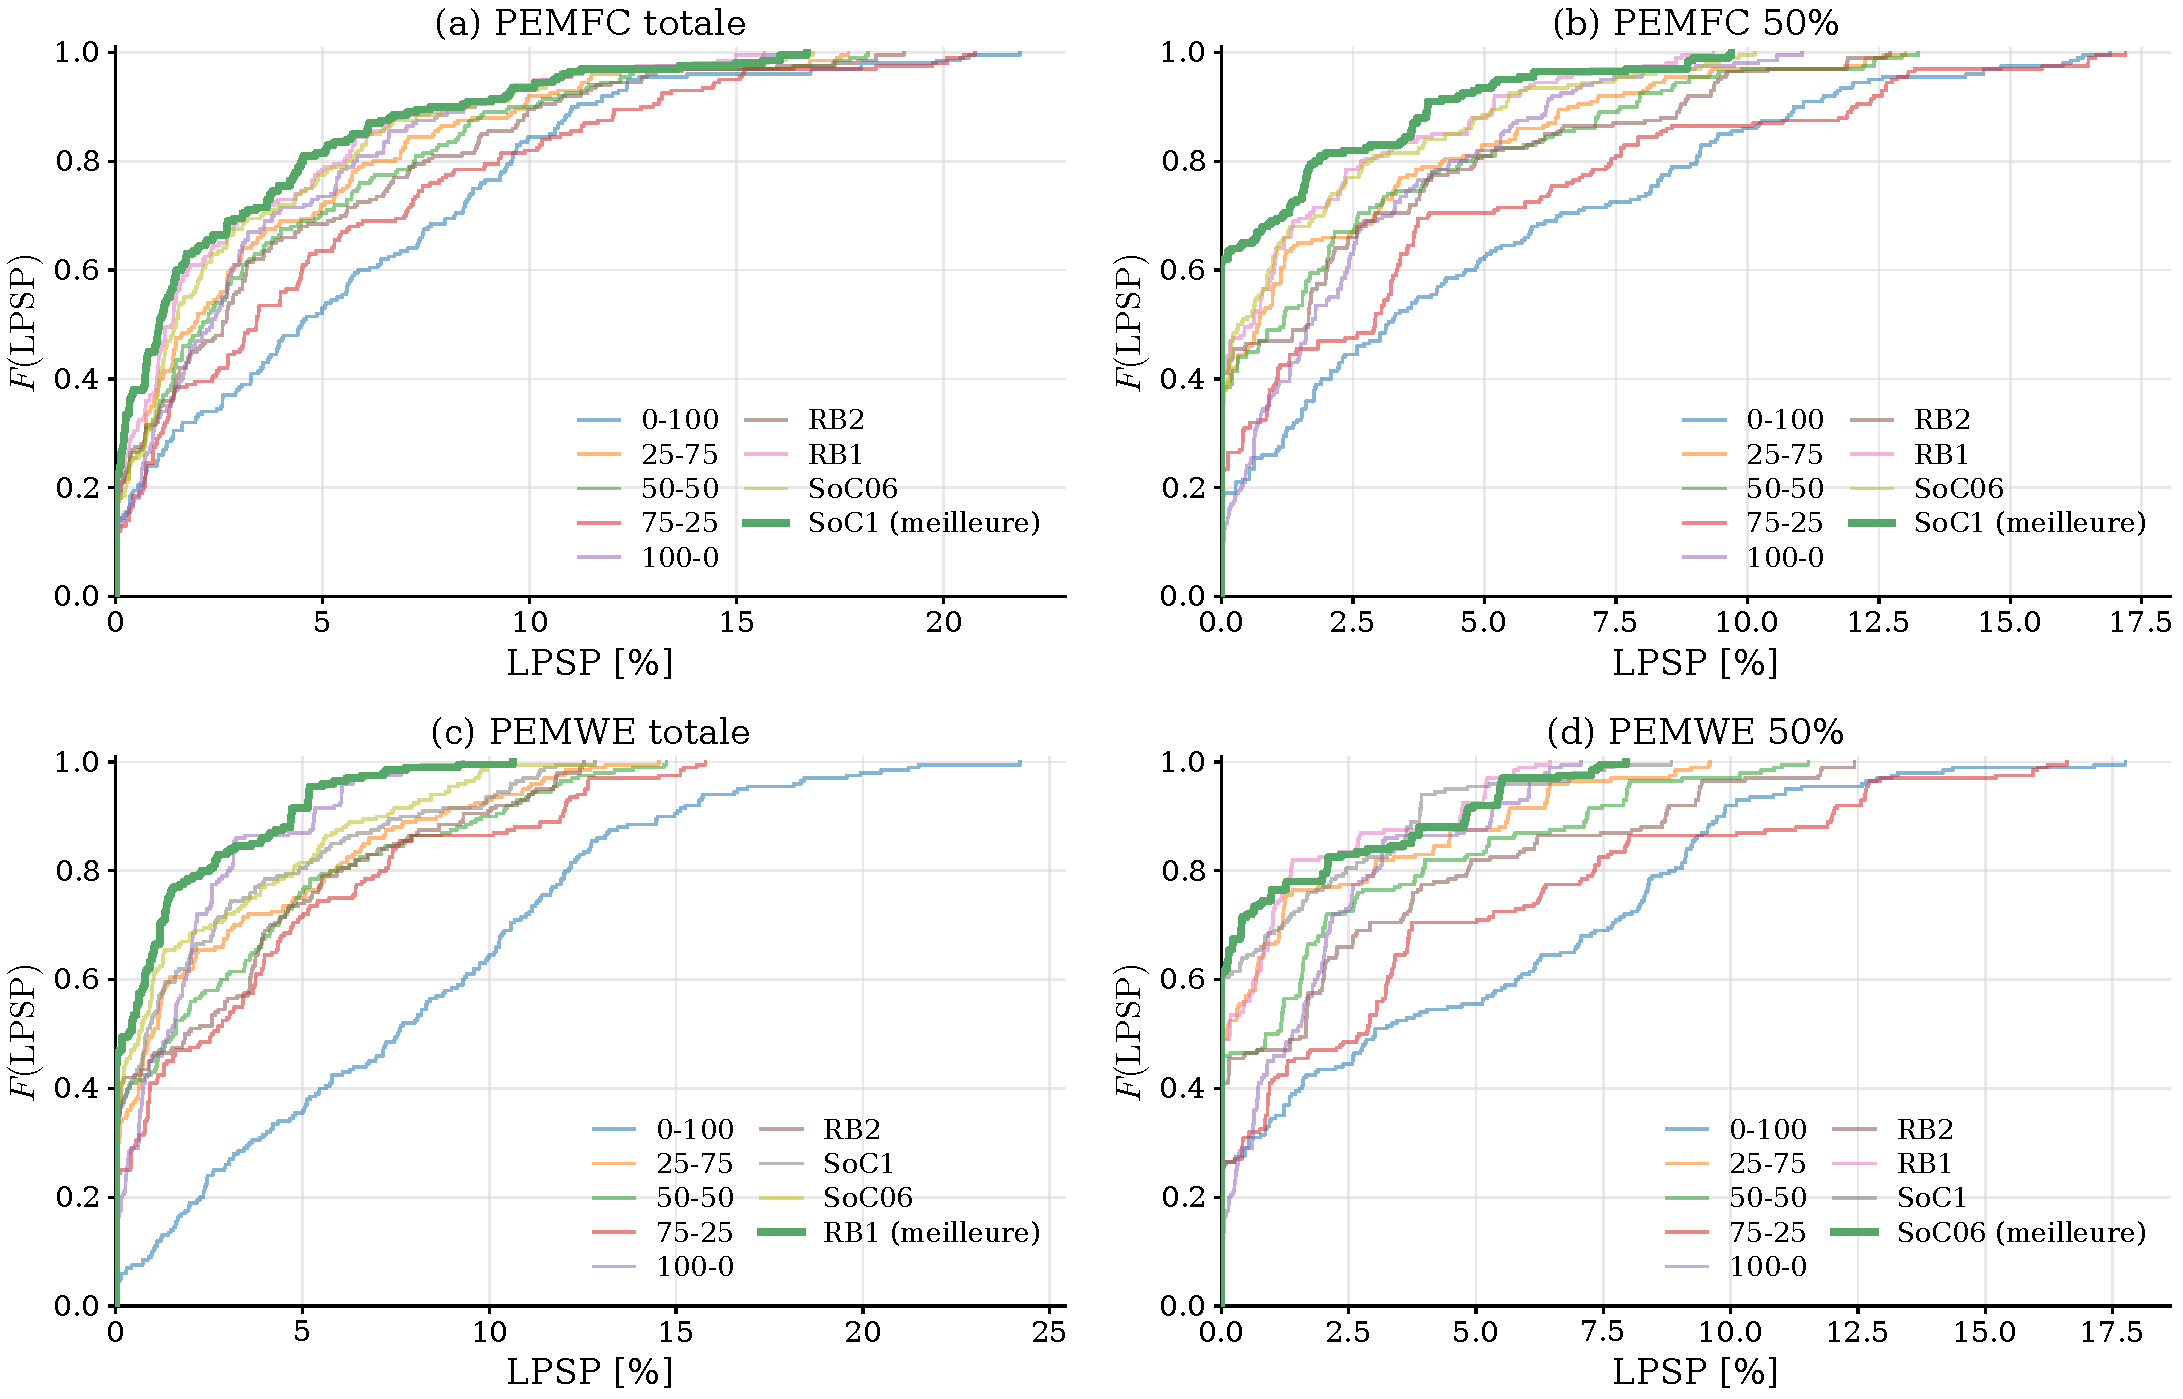
\includegraphics[width=\linewidth]{Chapitre 2/Robustesse/Figures/robustesse_cdf.pdf}
    \caption{Fonctions de répartition de la LPSP sous défaillance, par scénario.}
    \label{fig:rob_cdf}
\end{figure}
\FloatBarrier

% ------------------------------------------------------------
\subsubsection{Discussion}
% ------------------------------------------------------------

Le principal enseignement de cette analyse est qu'aucune stratégie ne domine simultanément les trois axes de performance. Les stratégies les plus robustes en LPSP absolue (SoC1, RB1) sont aussi parmi les plus coûteuses en dégradation, SoC1 culminant à 141~k€ sur le plan de Pareto, précisément parce que la forte réserve d'énergie qui les protège des pannes est obtenue au prix d'une sollicitation intense des composants hydrogène. Réciproquement, la stratégie 0-100, qui n'est pas la plus mauvaise sur le plan de Pareto nominal, se révèle la plus fragile face aux défaillances. La robustesse constitue donc une dimension de performance distincte, non réductible au compromis entre LPSP et dégradation, et qui mérite d'être évaluée explicitement.

La lecture des quatre scénarios met par ailleurs en évidence une asymétrie entre les deux composants hydrogène et entre les deux sévérités. La défaillance de la pile à combustible se traduit immédiatement par un déficit de service~: la PAC étant le seul organe capable de restituer l'énergie stockée sous forme d'hydrogène en période de déficit, sa perte ne peut être compensée que par la batterie, dont la réserve devient alors déterminante. La défaillance de l'électrolyseur n'a en revanche pas d'effet immédiat sur la satisfaction de la charge~: le surplus PV qui ne peut plus être électrolysé est simplement réorienté vers la batterie ou écrêté, sans coupure. Son coût est différé~: faute de pouvoir reconstituer le stock d'hydrogène pendant la panne, le réservoir s'appauvrit et la pile à combustible finit par manquer de carburant. C'est pourquoi la LPSP est évaluée sur une fenêtre incluant la reprise post-réparation, comme discuté à la section~\ref{subsec:indic_robustesse}. Les défaillances partielles (\SI{50}{\percent}) sont quant à elles bien mieux encaissées que les pannes totales~: la capacité résiduelle suffit souvent à couvrir une part substantielle de la demande, ce qui ramène le surcoût à des valeurs faibles voire négligeables, en particulier pour l'électrolyseur.

Les surcoûts très faibles relevés pour les défaillances partielles, en particulier celle de l'électrolyseur, pourraient laisser croire à un surdimensionnement des composants. Cette lecture serait toutefois trompeuse. Un électrolyseur dimensionné, par exemple, moitié plus petit ne dégraderait pas nécessairement la LPSP (sa capacité résiduelle resterait souvent suffisante pour absorber le surplus photovoltaïque), mais il fonctionnerait en permanence à une puissance relative bien plus élevée, et serait donc davantage exposé aux mécanismes d'usure liés au fonctionnement soutenu à forte charge. La bonne tenue apparente sous défaillance partielle ne saurait donc justifier un sous-dimensionnement, qui se paierait en durabilité.

Sur le plan opérationnel, ces résultats convergent vers une recommandation simple~: une réserve de batterie suffisante constitue la principale marge de robustesse d'un tel système isolé. Les stratégies qui épuisent ou immobilisent cette réserve, en la maintenant artificiellement haute au prix d'une forte sollicitation hydrogène (SoC1) ou en s'en remettant presque exclusivement à l'hydrogène (0-100), sont les plus pénalisées lors d'une panne. Toute stratégie conservant une marge de batterie mobilisable transforme à l'inverse cette marge en assurance face aux défaillances. Ce constat plaide aussi, en pratique, pour un léger surdimensionnement de la batterie et pour une maintenance préventive ciblant en priorité la pile à combustible, dont la défaillance est la plus immédiatement pénalisante.

Un autre point central mérite d'être souligné~: les défaillances considérées sont supposées mesurables, c'est-à-dire détectées par la supervision dès leur apparition. Cette hypothèse est raisonnable pour des composants instrumentés, dont la mise hors service ou le dérating est directement observable. Rien n'oblige alors à conserver, pendant la panne, la stratégie employée en régime nominal. Dès qu'une défaillance est détectée, la supervision peut basculer, le temps de l'indisponibilité, vers la stratégie qui minimise la LPSP dans le scénario rencontré (Figure~\ref{fig:rob_heatmap}), avant de revenir au régime nominal après réparation. L'analyse de robustesse ne désigne donc pas une stratégie unique~: elle fournit, pour chaque type de panne, la stratégie de repli la plus appropriée. Ces résultats ne remettent pas en cause le choix de la stratégie nominale issu du plan de Pareto, qui demeure de mise en fonctionnement normal et servira de point de départ à l'approche anticipative du chapitre suivant~; ils le complètent d'une politique de repli activée à la détection d'une panne.

Cette étude appelle néanmoins quelques réserves méthodologiques. La panne est ici supposée parfaitement détectée et instantanément prise en compte par le répartiteur~; un retard de détection ou un diagnostic erroné dégraderait les performances, en particulier pour les stratégies les plus dépendantes du composant défaillant. Par ailleurs, seules les défaillances des composants hydrogène ont été considérées et la durée de panne a été fixée à une semaine~; l'extension à des défaillances de batterie, à des durées variables ou à des pannes simultanées constitue une perspective naturelle. Enfin, la robustesse a été évaluée à travers la seule LPSP~; elle pourrait être complétée par un coût de la charge non desservie, dans l'esprit du critère de coût total unifié introduit à la section suivante.